De registry is een database die settings bevat voor Windows of applicaties die gekozen hebben om hun settings op te slaan in de regsitry. Meestal zijn dit low-level settings. Via de Registry Editor kan je deze settings aanpassen, verwijderen of toevoegen. De Registry Editor geeft je de mogelijkheid om ook settings die niet op een andere manier aangepast kunnen worden te wijzigen. Er is natuurlijk een goede reden dat deze settings zo verborgen zitten. Een waarschuwing is hier dan ook op zijn plaats: weet wat je doet! Wijzigingen in de registry kunnen je systeem instabiel maken, applicaties doen crashen en er zelfs voor zorgen dat Windows niet meer opstart. Zorg er dus voor dat je een backup hebt van de registry voordat je wijzigingen aanbrengt en wijzig alleen die zaken waarvan je absoluut zeker bent!

Om de Registry Editor te openen:
\begin{itemize}
\item Klik op het zoek icoon en zoek op Registry Editor
\item Gebruik de windows-toets + r en run regedit
\end{itemize}

\begin{minipage}[t]{\linewidth}
\raggedright
\adjustbox{valign=t}{%
	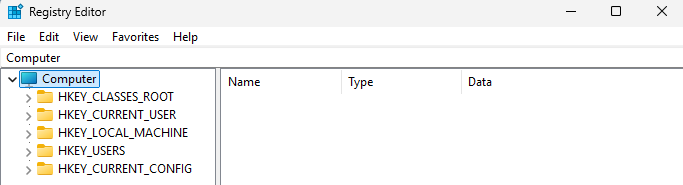
\includegraphics[width=0.99\linewidth]{regedit.png}%
}
\end{minipage}

